%% LyX 2.2.0 created this file.  For more info, see http://www.lyx.org/.
%% Do not edit unless you really know what you are doing.
\documentclass[11pt,american,handout]{beamer}
\usepackage{lmodern}
\renewcommand{\sfdefault}{lmss}
\renewcommand{\ttdefault}{lmtt}
\usepackage[T1]{fontenc}
\usepackage[utf8]{inputenc}
\setcounter{secnumdepth}{3}
\setcounter{tocdepth}{3}
\usepackage{array}
\usepackage{amssymb}
\usepackage{graphicx}

\makeatletter

%%%%%%%%%%%%%%%%%%%%%%%%%%%%%% LyX specific LaTeX commands.
\pdfpageheight\paperheight
\pdfpagewidth\paperwidth

%% Because html converters don't know tabularnewline
\providecommand{\tabularnewline}{\\}

%%%%%%%%%%%%%%%%%%%%%%%%%%%%%% Textclass specific LaTeX commands.
 % this default might be overridden by plain title style
 \newcommand\makebeamertitle{\frame{\maketitle}}%
 % (ERT) argument for the TOC
 \AtBeginDocument{%
   \let\origtableofcontents=\tableofcontents
   \def\tableofcontents{\@ifnextchar[{\origtableofcontents}{\gobbletableofcontents}}
   \def\gobbletableofcontents#1{\origtableofcontents}
 }
 % plain title style, override default
 \renewcommand\makebeamertitle{\frame[plain]{\maketitle}}%

%%%%%%%%%%%%%%%%%%%%%%%%%%%%%% User specified LaTeX commands.
\usepackage{microtype}
\usetheme{Frankfurt}
\usepackage{tikz}
\usepackage{bm}
\usepackage{animate}
\usepackage[absolute,overlay]{textpos}
\usetikzlibrary{automata,positioning,arrows.meta}
\setbeamertemplate{navigation symbols}{}
\useoutertheme{split}
\usepackage{ae,aecompl}
\usepackage{algorithmic}
\deftranslation[to=italian]{Definition}{Definizione}
\deftranslation[to=italian]{Examples}{Esempi}
\deftranslation[to=italian]{Example}{Esempio}
\deftranslation[to=italian]{Theorem}{Teorema}
\deftranslation[to=italian]{Corollary}{Corollario}
\definecolor{blue1}{RGB}{51,51,179}
\definecolor{blue2}{RGB}{0,0,204}
\definecolor{blue3}{RGB}{0,0,153}
\setbeamercolor{author in head/foot}{fg=white, bg=blue3}
\setbeamercolor{title in head/foot}{fg=white, bg=blue2}
\setbeamercolor{date in head/foot}{fg=white, bg=blue1}
\setbeamertemplate{navigation symbols}{}
\setbeamertemplate{footline}
{
  \leavevmode%
  \hbox{%
  \begin{beamercolorbox}[wd=.333333\paperwidth,ht=2.25ex,dp=1ex,center]{author in head/foot}%
    \usebeamerfont{author in head/foot}\insertshortauthor~~\beamer@ifempty{\insertshortinstitute}{}{(\insertshortinstitute)}
  \end{beamercolorbox}%
  \begin{beamercolorbox}[wd=.333333\paperwidth,ht=2.25ex,dp=1ex,center]{title in head/foot}%
    \usebeamerfont{title in head/foot}\insertshorttitle
  \end{beamercolorbox}%
  \begin{beamercolorbox}[wd=.333333\paperwidth,ht=2.25ex,dp=1ex,right]{date in head/foot}%
    \usebeamerfont{date in head/foot}\insertshortdate{}\hspace*{2em}
    \insertframenumber{} / \inserttotalframenumber\hspace*{2ex} 
  \end{beamercolorbox}}%
  \vskip0pt%
}
\setbeamersize{text margin left=1cm,text margin right=1cm} 

\makeatother

\usepackage{babel}
\begin{document}

\title{Chordal graphs: a linear testing algorithm}

\author{Gabriele Vanoni}

\institute{Politecnico di Milano}

\date{14 June 2017}
\makebeamertitle
\begin{frame}{Motivations}
\begin{itemize}
\item Many problems are in general \textbf{NP}-hard for graphs. For example
find Hamiltonian cycles or maximal cliques.
\item On particular classes of graphs though these problems can become low-degree
polynomial.
\item Chordal graphs are one of those classes for which many \textbf{NP}-hard
problems become low-degree polynomial (e.g. maximal cliques).
\item At this point become important that testing chordality is itself low-degree
polynomial.
\end{itemize}
\end{frame}

\section{The algorithm}
\begin{frame}[plain]
\begin{center}
\textbf{\LARGE{}The algorithm}
\par\end{center}{\LARGE \par}

\end{frame}
\begin{frame}{Preliminary definitions}

\vspace{-0.1cm}

\begin{definition}[Undirected graph]
A \textit{graph} $G$ is a pair $(V,E)$ where $V$ is a finite set
and $E$ is a set of $2-$subsets of $V$. Elements of $V$ are called
\textit{vertices} while elements of $E$ are called \textit{edges}.
$\left|V\right|=n$, $\left|E\right|=m$.\pause
\end{definition}

\begin{definitions}[Path, Cycle, Chord]
\begin{itemize}
\item A \textit{path} $\pi$ is a sequence of distinct vertices $v_{1},v_{2},\cdots v_{i},\cdots,v_{k}$
where $\{v_{i},v_{i+1}\}\in E$ with $1\leq i<k$.\pause
\item A \textit{cycle} of lenght $k+1$ is a closed path, i.e. a path for
which $\{v_{1},v_{k}\}\in E$.\pause
\item A \textit{chord} is an edge connecting two nonconsecutive vertices
of a cycle.\pause
\end{itemize}
\end{definitions}

\begin{definition}[Chordal graph]
A graph is chordal if every cycle of lenght at least four has a chord.
\end{definition}

\end{frame}
%
\begin{frame}{Orderings and fill-ins}
\begin{definition}[Ordering]
An \textit{ordering} is a bijection $\alpha:V\rightarrow\{1,2,\cdots,n\}$.
$v<_{\alpha}w$ iff $V(v)<V(w)$.\pause
\end{definition}

\begin{definition}[Fill-in]
A \textit{fill-in} induced by an ordering $\alpha$ is a set of edges
$F(\alpha)\not\in E$ such that there exists a path containing only
$u,v$ and vertices ordered after both $u$ and $v$. $F(\alpha)$
is \textit{zero fill-in} if $F(\alpha)=\varnothing$ and $\alpha$
is a zero fill-in ordering.\pause

\end{definition}

\begin{definition}[Elimination graph]
The \textit{elimination graph} of $G$ w.r.t. the ordering $\alpha$
is $G(\alpha)=(V,E\cup F(\alpha))$.
\end{definition}

\end{frame}
%
\begin{frame}{Example}

\begin{columns}
		\begin{column}{5cm}
			\centering
			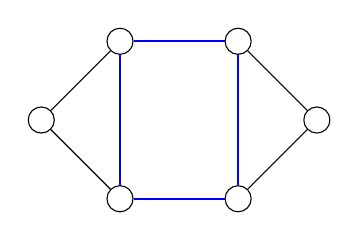
\begin{tikzpicture}
				\draw (0,1) node[draw, circle] (a) {};
				\draw (1,0) node[draw, circle] (b) {};
				\draw (1,2) node[draw, circle] (c) {};
				\draw (2.5,0) node[draw, circle] (d) {};
				\draw (2.5,2) node[draw, circle] (e) {};
				\draw (3.5,1) node[draw, circle] (f) {};
			
				\draw (c) -- (a) -- (b);
				\draw (d) -- (f) -- (e);
				\draw[blue, line width = 0.3mm] (b) -- (c) -- (e) -- (d) -- (b);
			\end{tikzpicture}\newline
			not chordal \vspace{0.7cm}
			

			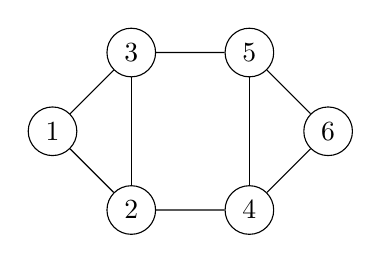
\begin{tikzpicture}
				\draw (0,1) node[draw, circle] (a) {1};
				\draw (1,0) node[draw, circle] (b) {2};
				\draw (1,2) node[draw, circle] (c) {3};
				\draw (2.5,0) node[draw, circle] (d) {4};
				\draw (2.5,2) node[draw, circle] (e) {5};
				\draw (3.5,1) node[draw, circle] (f) {6};
			
				\draw (a) -- (b) -- (d) -- (f) -- (e) -- (c) -- (a);
				\draw (b) -- (c);
				\draw (d) -- (e);
			\end{tikzpicture}\newline
			ordered
		\end{column}
		\begin{column}{5cm}
			\centering
			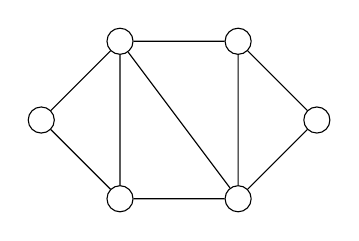
\begin{tikzpicture}
				\draw (0,1) node[draw, circle] (a) {};
				\draw (1,0) node[draw, circle] (b) {};
				\draw (1,2) node[draw, circle] (c) {};
				\draw (2.5,0) node[draw, circle] (d) {};
				\draw (2.5,2) node[draw, circle] (e) {};
				\draw (3.5,1) node[draw, circle] (f) {};
			
				\draw (a) -- (b) -- (d) -- (f) -- (e) -- (c) -- (a);
				\draw (b) -- (c) -- (d) -- (e);
			\end{tikzpicture}\newline
			chordal\vspace{0.7cm}
				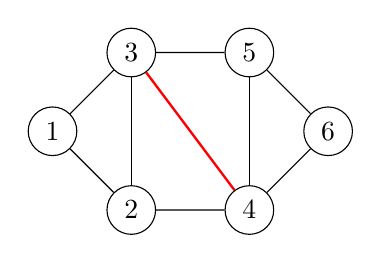
\begin{tikzpicture}
				\draw (0,1) node[draw, circle] (a) {1};
				\draw (1,0) node[draw, circle] (b) {2};
				\draw (1,2) node[draw, circle] (c) {3};
				\draw (2.5,0) node[draw, circle] (d) {4};
				\draw (2.5,2) node[draw, circle] (e) {5};
				\draw (3.5,1) node[draw, circle] (f) {6};
			
				\draw (a) -- (b) -- (d) -- (f) -- (e) -- (c) -- (a);
				\draw (b) -- (c);
				\draw (d) -- (e);
				\draw[red, line width = 0.3mm] (c) -- (d);
			\end{tikzpicture}\newline
			elimination graph
		\end{column}
	\end{columns}
\end{frame}
%
\begin{frame}{Testing chordality}
\begin{theorem}
A graph is chordal if and only if it has a zero fill-in ordering.\pause
\end{theorem}

We want to compute an ordering $\alpha$ that is zero fill-in if and
only if $G$ is chordal. In this way we can compute $F(\alpha)$.
$G$ is chordal if and only if $F(\alpha)=\varnothing$.\pause
\begin{definition}[Maximum cardinality search (MCS)]
It's an ordering algorithm in which at each step $i$ (from $1$
to $n$) the vertex selected and numberd with $i$ among the unnumbered
ones is that adjacent to the largest number of previously numberd
vertices, breaking ties arbitrarily.\pause
\end{definition}

\begin{theorem}
An ordering generated by MCS is zero fill-in if the graph is chordal.

\end{theorem}

\end{frame}
%
\begin{frame}{MCS - complexity analysis}

\begin{textblock}{50}(7.7,2.1)

{\footnotesize{}\begin{algorithmic}[1]
\FOR{$i=0$ \TO $n-1$ } {
	\STATE $set[i]:=\varnothing$ }
\ENDFOR
\FORALL{ $v$ in $V$} {
	\STATE $size[v]:=0;\,set[0]:=set[0]\cup\{v\}$ }
\ENDFOR
\STATE $j:=0$
\FOR {$i=1$ \TO $n$ } {
	\STATE $v:=$ delete any node from $set[j]$
	\STATE $\alpha [v]:=i;\,\alpha^{-1} [i]:=v;\,size[v]:=-1$
	\FORALL {$(u,v)\in E$ and $size[u]\geq 0$} {
		\STATE delete $u$ from $set[size[u]]$
		\STATE $size[u]:=size[u]+1$
		\STATE $set[size[u]]:=set[size[u]]\cup \{u\}$ }
	\ENDFOR }
	\STATE $j:=j+1$
	\WHILE {$j\geq 0$ and $set[j]=\varnothing$} {
		\STATE $j:=j-1$ }
	\ENDWHILE
\ENDFOR
\end{algorithmic}}{\footnotesize \par}

\end{textblock}

\begin{textblock}{6}(1,2.1)
\begin{theorem}
Complexity of the algorithm that computes the MCS ordering is $\mathcal{O}(n+m)$.
\end{theorem}

\begin{proof}
The first two for loops are $\mathcal{O}(n)$. The third is also $\mathcal{O}(n)$
but there are inner loops. However in the first one every edge is
scanned at most twice, while the second one is executed at most $n$
times yielding a total cost of the outer loop of $\mathcal{O}(n+m)$.
\end{proof}

\end{textblock}
\end{frame}
%
\begin{frame}{Computing the fill-in}
\begin{definition}
The \textit{follower} of a vertex $v$, $f(v)$ is the vertex $w$
of largest number (w.r.t to $\alpha$) both adjacent to $v$ in $G(\alpha)$
and such that $w<_{\alpha}v$. For $i\geq0$, $f^{0}(v)=v$ and $f^{i+1}(v)=f(f^{i}(v))$.\pause
\end{definition}

\begin{theorem}
If $x,w\in V$ with $w<_{\alpha}x$, then $(x,w)\in E\cup F(\alpha)$
if and only if there is a vertex $v$ such that $(v,w)\in E$ and
$f^{i}(v)=x$ for some $i\geq0$.\pause
\end{theorem}

With this theorem we can compute for any vertex $w$, the set $A(w)=\{x|(x,w)\in E\cup F(\alpha),$$w<_{\alpha}x\}$
and also all vertices $x$ such that $f(x)=w$.

\end{frame}
%
\begin{frame}{Computing the fill-in - complexity analysis}

\begin{textblock}{50}(7.5,3.2)

{\footnotesize{}\begin{algorithmic}[1]
\FOR{$i=n$ \TO $1$ } {
	\STATE $w:=\alpha^{-1}[i]$
	\STATE $f[w]:=w$
	\STATE $index[w]:=i$
	\FORALL {$v\in V$ s.t. $(v,w)\in E$ and $\alpha [v]>i$} {
		\STATE $x:=v$
		\WHILE {$index[x]>i$} {
			\STATE $index[x]:=i$
			\STATE add $(x,w)$ to $E\cup F(\alpha)$
			\STATE $x:=f[x]$
		}\ENDWHILE
		\IF {$f[x]=x$} {
			\STATE $f[x]:=w$ }
		\ENDIF }
	\ENDFOR }
\ENDFOR
\end{algorithmic}}{\footnotesize \par}

\end{textblock}

\begin{textblock}{6}(1,2.8)
\begin{theorem}
Complexity of the algorithm that computes the fill-in of a graph $G$
is $\mathcal{O}(n+m')$ where $m'=|E\cup F(\alpha)|$.
\end{theorem}

\begin{proof}
The outer loop is executed $n$ times. The inner one is scans each
vertex of the elimination graph at most twice yielding a total cost
of the outer loop of $\mathcal{O}(n+m')$.
\end{proof}

\end{textblock}
\end{frame}
%
\begin{frame}{Testing cordality - complexity analysis}

\begin{textblock}{50}(7.5,3.2)

{\footnotesize{}\begin{algorithmic}[1]
\FOR{$i=n$ \TO $1$ } {
	\STATE $w:=\alpha^{-1}[i]$
	\STATE $f[w]:=w$
	\STATE $index[w]:=i$
	\FORALL {$v\in V$ s.t. $(v,w)\in E$ and $\alpha [v]>i$} {
		\STATE $x:=v$
		\WHILE {$index[x]>i$} {
			\STATE $index[x]:=i$
			\IF {$(x,w)\not\in E$ and $x\neq w$} {
				\RETURN false }
			\ENDIF
			\STATE $x:=f[x]$
		}\ENDWHILE
		\IF {$f[x]=x$} {
			\STATE $f[x]:=w$ }
		\ENDIF }
	\ENDFOR }
\ENDFOR
\RETURN true
\end{algorithmic}}{\footnotesize \par}

\end{textblock}

\begin{textblock}{6}(1,2.8)
\begin{theorem}
Complexity of the algorithm that recognizes cordality of a graph $G$
is $\mathcal{O}(n+m)$.
\end{theorem}

\begin{proof}
The outer loop is executed $n$ times. The inner one is scans each
vertex of the $G$ at most twice yielding a total cost of the outer
loop of $\mathcal{O}(n+m)$.
\end{proof}

\end{textblock}
\end{frame}

\section{Implementation}
\begin{frame}[plain]
\begin{center}
\textbf{\LARGE{}Implementation}
\par\end{center}{\LARGE \par}

\end{frame}
\begin{frame}{Language and libraries}
\begin{itemize}
\item \textbf{JavaSE 8} was used to implement the algorithm.
\item Graph data structures were provided by \textbf{JUNG} library and graphs
were stored in \textbf{PajekNet} format.
\item \textbf{Apache Maven} was used to handle the project.
\item \textbf{Eclipse} was used as IDE.
\item The code is released under \textbf{GPL 3} license.
\item \textbf{Oracle Java Mission Control} with \textbf{Flight Recorder}
was used to profile the application.
\end{itemize}
\end{frame}
%
\begin{frame}{Data structures}

Two data structures were defined to implement the algorithms.
\begin{block}{Vertex}
\begin{itemize}
\item \texttt{alpha:int}
\item \texttt{size:int}
\item \texttt{index:int}
\item \texttt{follower:Vertex\pause}
\end{itemize}
\end{block}
%
\begin{block}{ChordalAlgorithms}
\begin{itemize}
\item \texttt{order:List<Vertex>}
\item \texttt{graph:UndirectedGraph<Vertex,Integer>}
\item \texttt{maximumCardinalitySearch():void}
\item \texttt{isChordal():boolean}
\end{itemize}
\end{block}
\end{frame}
%
\begin{frame}{Testing environment}
\begin{block}{}
\begin{itemize}
\item \textbf{JVM}: Oracle 1.8.0\_111-b14
\item \textbf{OS}: Ubuntu 15.10
\item \textbf{Linux kernel}: 4.2.0-42-generic
\item \textbf{libc}: glibc 2.21
\item \textbf{System architecture}: x86\_64
\item \textbf{CPU}: Intel Core i7-2600K CPU @ 3.40GHz
\item \textbf{Memory}: 8 GB
\end{itemize}
\end{block}
\end{frame}
%
\begin{frame}{Datasets}
\begin{itemize}
\item I chose to use \textbf{real networks} data to test the algorithms\footnote{\texttt{http://vlado.fmf.uni-lj.si/pub/networks/data/}; M. Boguña,
R. Pastor-Satorras, A. Diaz-Guilera and A. Arenas, Physical Review
E, vol. 70, 056122 (2004)}.
\item All graphs from datasets were obviously non chordal.
\item For every datasets, I computed the elimination graph, so to have a
chordal graph and I exported it.
\item To measure performances I used only chordal graphs so that the complexity
is $\Theta(n+m)$.
\end{itemize}
\end{frame}
%
\begin{frame}{Profiling}

\textbf{\footnotesize{}Total time}{\footnotesize{} is the actual time
spent by the application to execute the two methods of the algorithm,
}\texttt{\footnotesize{}maximumCardinalitySearch()}{\footnotesize{}
and }\texttt{\footnotesize{}isChordal()}{\footnotesize{}. The data
structure }\texttt{\footnotesize{}ChordalAlgorithms}{\footnotesize{}
was already filled in with the graph read from file. Seven tests were
executed for each dataset.}{\footnotesize \par}
\begin{center}
{\scriptsize{}}%
\begin{tabular}{|c|c|c|c|}
\hline 
\textbf{\scriptsize{}Dataset} & \textbf{\scriptsize{}n+m} & \textbf{\scriptsize{}Total average time} & \textbf{\scriptsize{}Total minimum time}\tabularnewline
\hline 
\hline 
{\scriptsize{}YeastChordal} & {\scriptsize{}126547} & {\scriptsize{}328 ms} & {\scriptsize{}282 ms}\tabularnewline
\hline 
{\scriptsize{}PGPChordal} & {\scriptsize{}192058} & {\scriptsize{}608 ms} & {\scriptsize{}569 ms}\tabularnewline
\hline 
{\scriptsize{}MiniDaysAllChordal} & {\scriptsize{}2157699} & {\scriptsize{}9s 572 ms} & {\scriptsize{}9 s 711 ms}\tabularnewline
\hline 
{\scriptsize{}DaysAllChordal} & {\scriptsize{}3633865} & {\scriptsize{}19s 209 ms} & {\scriptsize{}18 s 103 ms}\tabularnewline
\hline 
\end{tabular}
\par\end{center}{\scriptsize \par}

\begin{center}
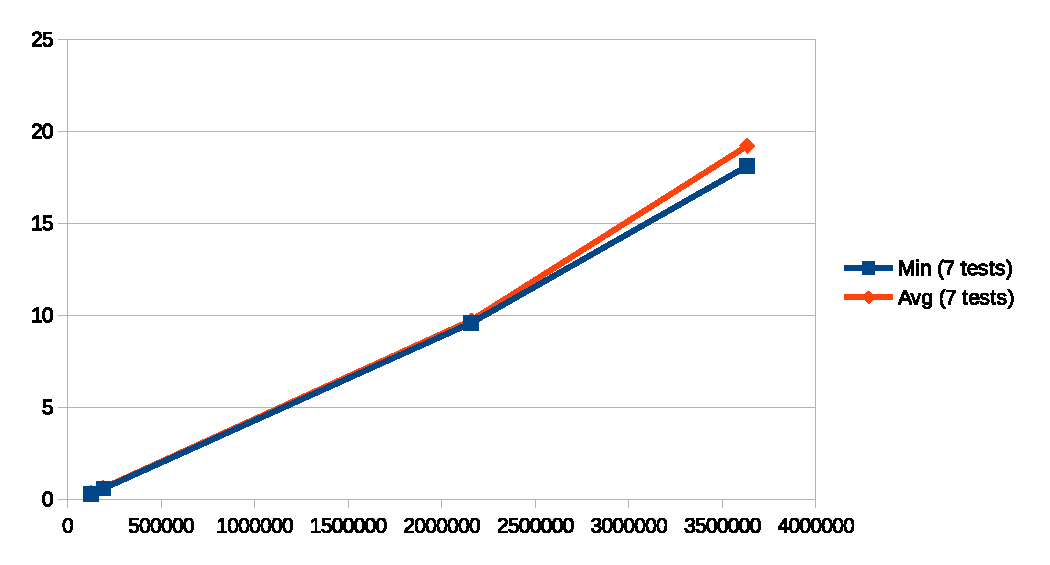
\includegraphics[scale=0.38]{img/plot}
\par\end{center}
\end{frame}

\section{Parallel versions}

\begin{frame}[plain]
\begin{center}
\textbf{\LARGE{}Parallel versions}
\par\end{center}{\LARGE \par}

\end{frame}
%
\begin{frame}{Parallel versions of the algorithm}

Recognizing chordal graphs is in the complexity class \textbf{NC},
as shown for the first time by Edenbrandt (1986), using a different
characterization of chordal graphs. After this seminal paper other
results were achieved in optimizing the algorithm.

\medskip{}

\begin{tabular}{|>{\centering}p{2.5cm}|c|>{\centering}m{2cm}|>{\centering}p{3cm}|}
\hline 
\textbf{Authors} & \textbf{Complexity} & \textbf{Number of processors} & \textbf{Cost model}\tabularnewline
\hline 
\hline 
Edenbrandt & $\mathcal{O}(\log n)$ & $\mathcal{O}(n^{5})$ & PRAM CREW\tabularnewline
\hline 
Chandrasekharan et al. & $\mathcal{O}(\log n)$ & $\mathcal{O}(n^{4})$ & PRAM CRCW\tabularnewline
\hline 
Klein & $\mathcal{O}(\log^{2}n)$ & $\mathcal{O}(n+m)$ & PRAM CRCW\tabularnewline
\hline 
Klein & $\mathcal{O}(\log^{2}n)$ & $\mathcal{O}(\frac{n+m}{\log n})$ & PRAM CRCW (randomized)\tabularnewline
\hline 
\end{tabular}

\end{frame}
%
\begin{frame}{Bibliografia}

{\footnotesize{}\bibliographystyle{plain}
\nocite{*}
\bibliography{ChordalGraphs}
}{\footnotesize \par}
\end{frame}

\end{document}
